%
% The first command in your LaTeX source must be the \documentclass command.
\documentclass[sigconf]{acmart}
%
% defining the \BibTeX command - from Oren Patashnik's original BibTeX documentation.
\def\BibTeX{{\rm B\kern-.05em{\sc i\kern-.025em b}\kern-.08emT\kern-.1667em\lower.7ex\hbox{E}\kern-.125emX}}
    
% Rights management information. 
% This information is sent to you when you complete the rights form.
% These commands have SAMPLE values in them; it is your responsibility as an author to replace
% the commands and values with those provided to you when you complete the rights form.
%



%%%%%%%%%%%%%%5
\usepackage{lipsum}


\begin{document}

%
% The "title" command has an optional parameter, allowing the author to define a "short title" to be used in page headers.
\title{Collaborating Agile Teams}

%
% The "author" command and its associated commands are used to define the authors and their affiliations.
% Of note is the shared affiliation of the first two authors, and the "authornote" and "authornotemark" commands
% used to denote shared contribution to the research.

\author{Trupti Khatavkar}
\email{tkhatavk@asu.edu}
\affiliation{%
  \institution{Arizona State University}
  \city{Tempe}
  \state{Arizona}
  \country{United States}
}

\author{Srajan Gupta}
\email{sgupt182@asu.edu}
\affiliation{%
  \institution{Arizona State University}
  \city{Tempe}
  \state{Arizona}
  \country{United States}
}

%
% The abstract is a short summary of the work to be presented in the article.
\begin{abstract}
Agile development model has its own advantages such as, flexibility, transperance, early and predictable delivery and it focuses on users. Taking this into consideration, large projects can be developed using agile techniques by dividing them into different components and distributing the components to different teams. This is generally termed as scrum of scrums. In such large project, each team should take the full responsibility of their own component and then the components are interfaced to build the whole system. The main challenge is to maintain minimum dependencies among teams as possible. This paper suggests methods to achieve successful large agile project. Also, methods to overcome architecure or design related risks are also put forward.
\end{abstract}


%
% Keywords. The author(s) should pick words that accurately describe the work being
% presented. Separate the keywords with commas.
\keywords{agile, components, dependencies, collaboration, communication}

%
% A "teaser" image appears between the author and affiliation information and the body 
% of the document, and typically spans the page. 


%
% This command processes the author and affiliation and title information and builds
% the first part of the formatted document.
\maketitle


\section{Introduction}
For developing any business, Software development is a core component \cite{HenrikK}. With great competition There has been a great investment in building high quality software. A software is developed in multi-site with multiple teams involved with a distributed environment. As discussed in \cite{4638656}Past few years, in order to allow changes and catch up with the new technology, the development community is using the agile software development, where the software develops gradually and this done between self-organizing cross-functional teams. 

This paper discusses some ways of achieving the practice of software development using agile method and the how different agile teams come together to build a software. It also dicusses the challenges which agile principles help in overcome in projects which are distibuted. Along with this, some of the techniques which can be incorporated in order to handle those challenges.

The paper is structured as follows : Section 2 discusses the methods of obtaining a large scale agile project which is distributed among many teams, what are some common practices to be followed among different team so that each one has the feel of the project, its design and architecture and agile software development methodology as well. Section 3 concludes it and list down some benefits of this software development process.


\section{Main}
\subsection{Methods to achieve successful large scale agile project}
The main challenges for working on a large project using multiple agile teams is communication, dependencies between components and interfacing those components. To achieve a successful project, following methods can be useful. 


\begin{itemize}
\item Separate Product Backlog for each team
\\As shown in Figure \ref{fig:PBCollab}, it is very important that every team should have a strong product backlog in agile when working in a distributed envirenment. But, clear separation of work is equally important. Every day to day operations should be separated among the teams. Overlapping situations should be planned during the cross team meetings.

\begin{figure}[H]
  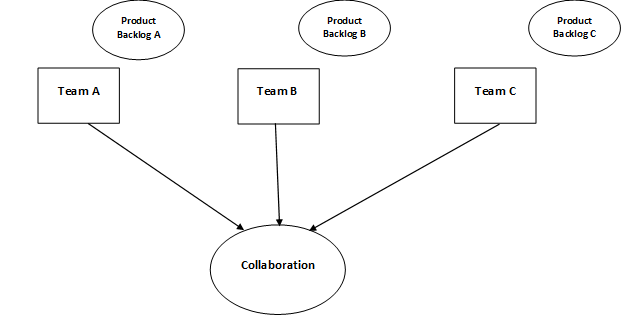
\includegraphics[width=0.5\textwidth]{PBCollab}
  \caption{Collaboration of teams and their backlogs.}
\Description{Teams collaborating to develop a single project}
  \label{fig:PBCollab}
\end{figure}

\item Tools for Interaction
\\Choosing the correct tool for communication matters when working in distributed agile environment. Slack and GitHub are very effective for this.

\item Agile Practices
\\All the important agile practices such as standups, planning, deliverables and retrospectives should be defined by each team as they think is suitable.

\item Face to face communication 
\\Using tools for communication is effective, but many times there are broken communications due to various technical issues such as poor connections, fault in the devices, etc. To overcome these, regular cross teams face to face communications are also important.
\end{itemize}

\subsection{Architecture/Design for distributed agile project}
Architecture defines the structure of the project. A well defined architecure makes a base for a succesful project. As multiple teams work on a single project, it is important to have a fixed architecture so that different teams can work on different components of the architecture. If there is no fixed single plan, interfacing of the components would be a difficult task. Also, the architecure can get messed up if multiple teams update it. The integrity of the whole project can be affected if architecture is messed up.


To overcome this problem, there should be a single Chief Architect (or two, working in a pair) who will guide the teams and ensures they do not stumble upon the architecure. Chief architect works on a high level architectural issues that involves all the components and inerfaces between them. 


Another method would be to crete the Architecture group. It is composed of each team's most skilled person. This group handles all the arcitectural issues rather than one person handling them. The group should not exceed more than 20 people, else communication problem arises. The group understands the subsystem's relationships and the architecure as a whole. Thus, the group decides how each team works and handles the project. 


\section{Conclusion}
With different teams working on a same project using the agile methodology, it is possible to make the best use of available talent across the organization and not outsourcing it while increasing the cost of the project. It is a conscious decision to include multiple teams in one project considering the different strategies, talent, focus and management of different teams can be factor in success, delivery time or may cause dysfunctioning but these factors needs to be clearly understood beforehanded.

There are many benefits of using different agile temas for software development. We can track the progess and evaluate the problems early in the stage, also handles the problem of isolated teams where there are difficulties in communication. It can help in sharing knowledge between different domains while different teams work together and look after the development with all aspects

With the benefits comes some challenges as well. Since there is informal communication in agile software development, it can lead to loss of information among teams and with this there can be a lack of trust. There is a lot of coordination required so that every team is on the same page and knows excatly at every step what is happening within the project. Each team should be making equal efforts towards the project development.

With proper coaching to themselves as a team is very important in collaborated development\cite{4638656}. Hence, with a little and right amount of modification in the existing agile techniques can be very helpful in overcoming the challenges faced and in term increase the production of high quality softwares.

% The next two lines define the bibliography style to be used, and the bibliography file.
\bibliographystyle{ACM-Reference-Format}%alpha
\bibliography{sample-base}

% 
% If your work has an appendix, this is the place to put it.
%\bibliography{sample-base}
\end{document}
